With the availability of our first synthetic dataset, the next step was to deploy \textsc{FedBiscuit} on EPFL's computing clusters in order to run the framework ourselves.

\section{Deployment on EPFL Clusters}

We started by copying the FedBiscuit repository on the SCITAS cluster and setting up an environment with the required dependencies. We quickly discovered that the original authors had run the framework on NVIDIA A100 GPUs, which support BF16 numerical precision. However, the SCITAS cluster uses NVIDIA V100 GPUs, which are not compatible with BF16.

As a result, we had to manually modify several hardcoded values in the code to replace BF16 with FP16. Once this was done, we faced a series of minor software engineering issues to ensure the framework could run correctly on the cluster environment.

Our objective was also to monitor the training runs using Weights \& Biases. To this end, we added compatibility with Weights \& Biases by integrating the tracking of key training variables such as hyperparameters, accuracy, and loss.

\section{Training Data Size Estimation}

Before launching full training runs on the synthetic dataset, we needed to determine how much data would be necessary to obtain meaningful results. To do this, we conducted a training data estimation experiment using the TL;DR summarization task proposed by the original authors in their paper.

The goal of this experiment was to identify the optimal dataset size that would yield strong performance with minimal training data. We fixed the number of clients in the federated setup to 52 and modified the client-side data processing logic to allow for a constant validation and test set, while varying the size of the training set across different experiments.

We kept the hyperparameters mostly aligned with the original setup, though we had to reduce the batch size from 8 to 1 in order to avoid CUDA out of memory error. We also reduced the number of federated rounds (from 500 to 150) to keep the training times manageable on the available infrastructure.

\section{Intermediary Results}

As of now, we do not yet have the evaluation results from the RLHF phase where the model is aligned using DPO with the Aggregated Binary Selector in the training data size estimation experiment. Therefore, our results are currently limited to the training metrics available through Weights \& Biases for the binary selectors training phase.

Below, we present some of the results related to the training of the binary selectors. We show the loss and accuracy on the validation set, followed by the corresponding metrics on the test set.  
It is important to note that, for each experiment, the validation and test sets were kept strictly identical to ensure fair comparison across runs.


\section{Challenges Encountered}

We faced numerous software engineering challenges during this process. One of the key issues was dependency compatibility: FedBiscuit is designed to run with Python 3.9, while the SCITAS environment enforces Python 3.10.4. This required us to manually adapt each dependency and resolve compatibility issues.

Another major challenge was training time. The V100 GPUs available on our cluster are significantly less powerful than the A100 GPUs used by the authors. Given the time constraints of the project, we were only able to train the binary selectors for all clients as part of the dataset size estimation experiment. However the RLHF trainings are still ongoing, and we will gather the results soon.

\begin{figure*}[h!]
	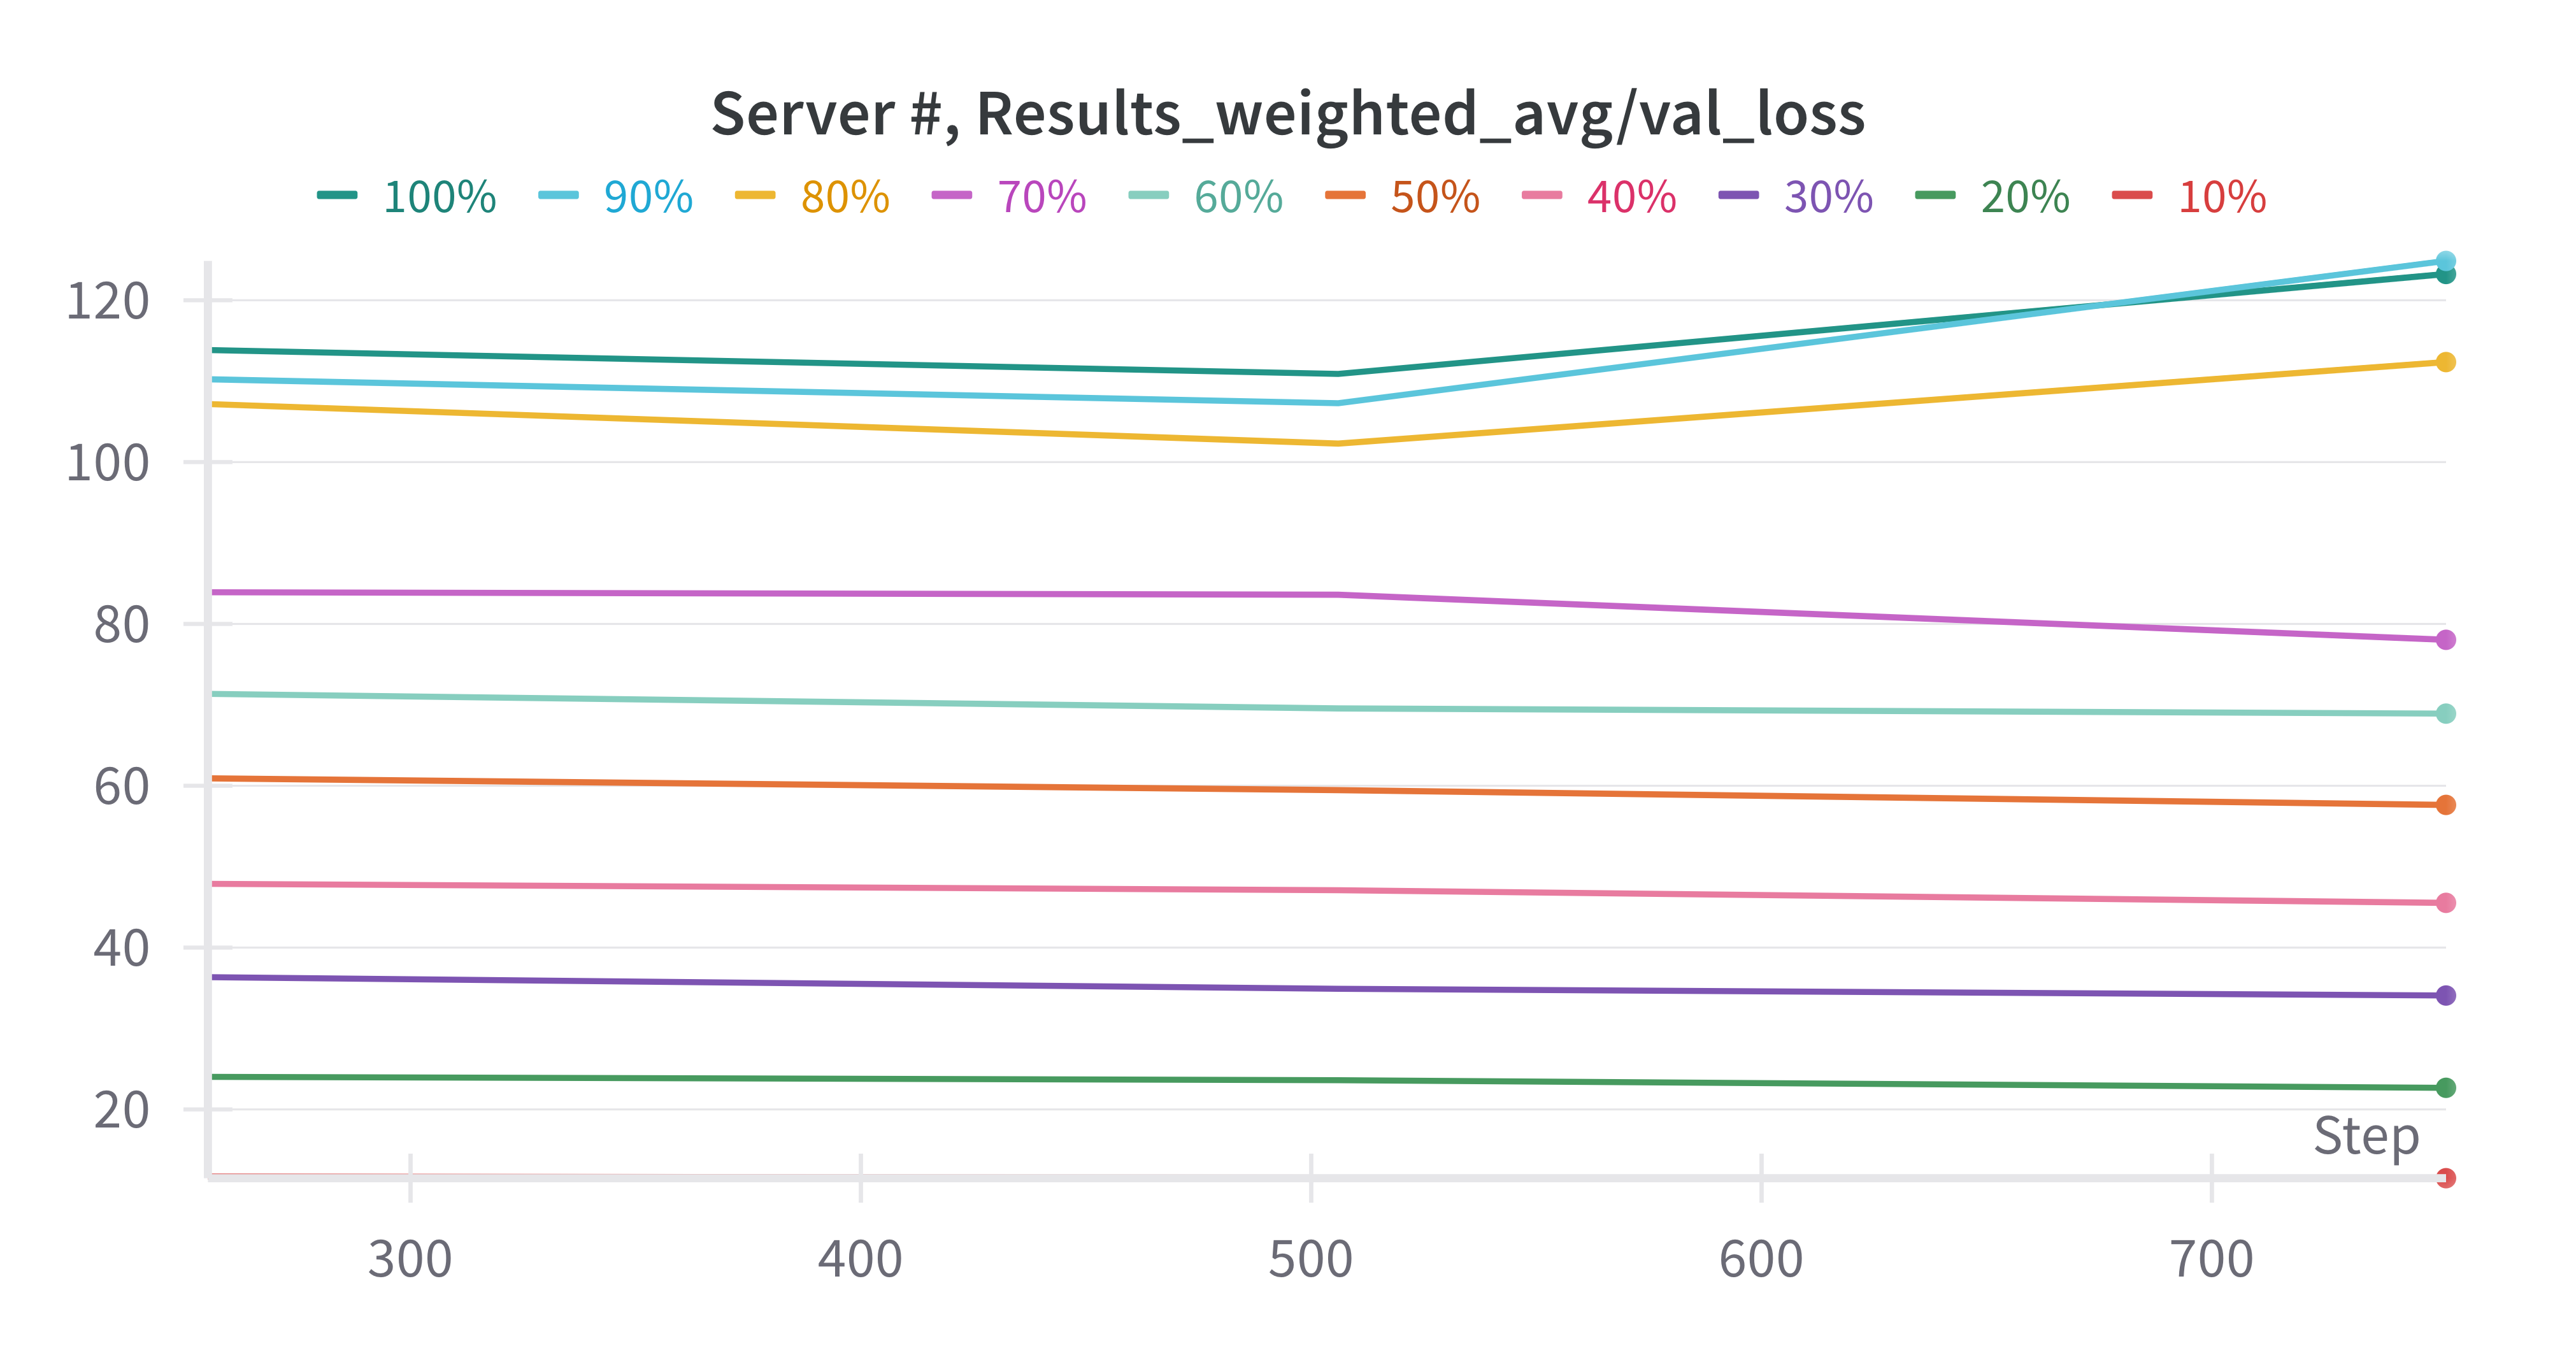
\includegraphics[width=\textwidth]{validation_loss}
  \caption{Plot of the average validation loss of the binary selectors across the different training set sizes.}
  \label{fig:v1}
\end{figure*}

\begin{figure*}[h!]
	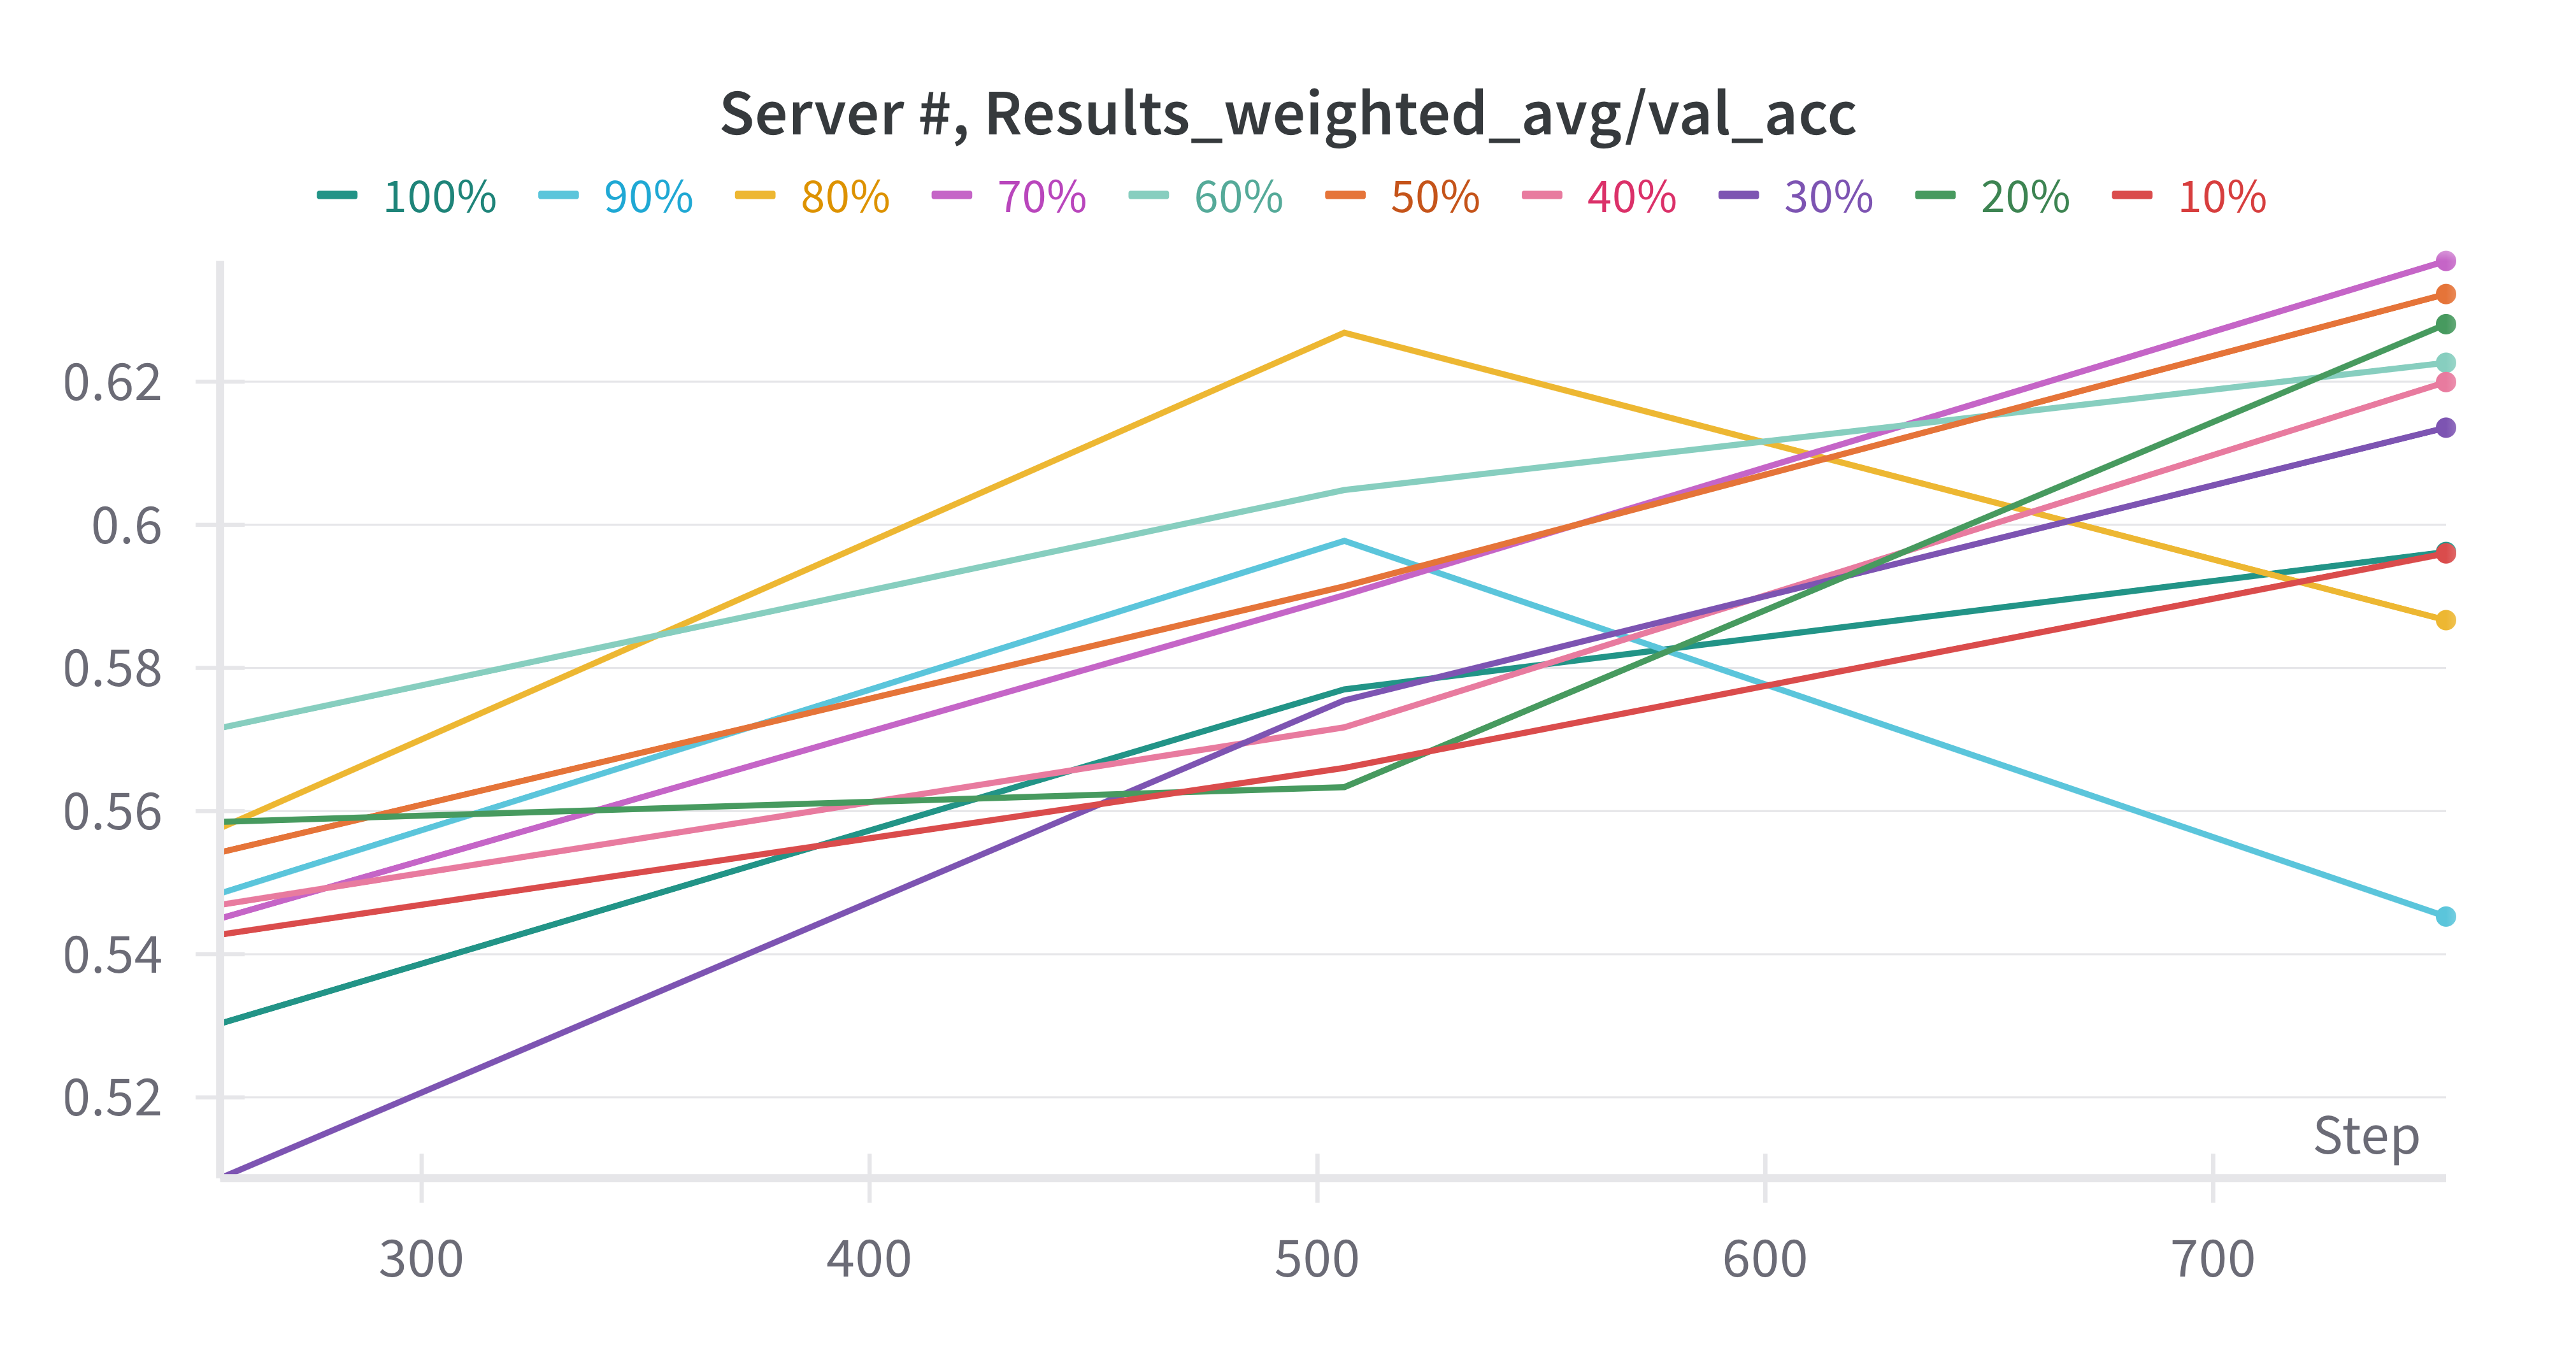
\includegraphics[width=\textwidth]{validation_acc}
  \caption{Plot of the average validation accuracy of the binary selectors across the different training set sizes.}
  \label{fig:v2}
\end{figure*}

\begin{figure*}[h!]
	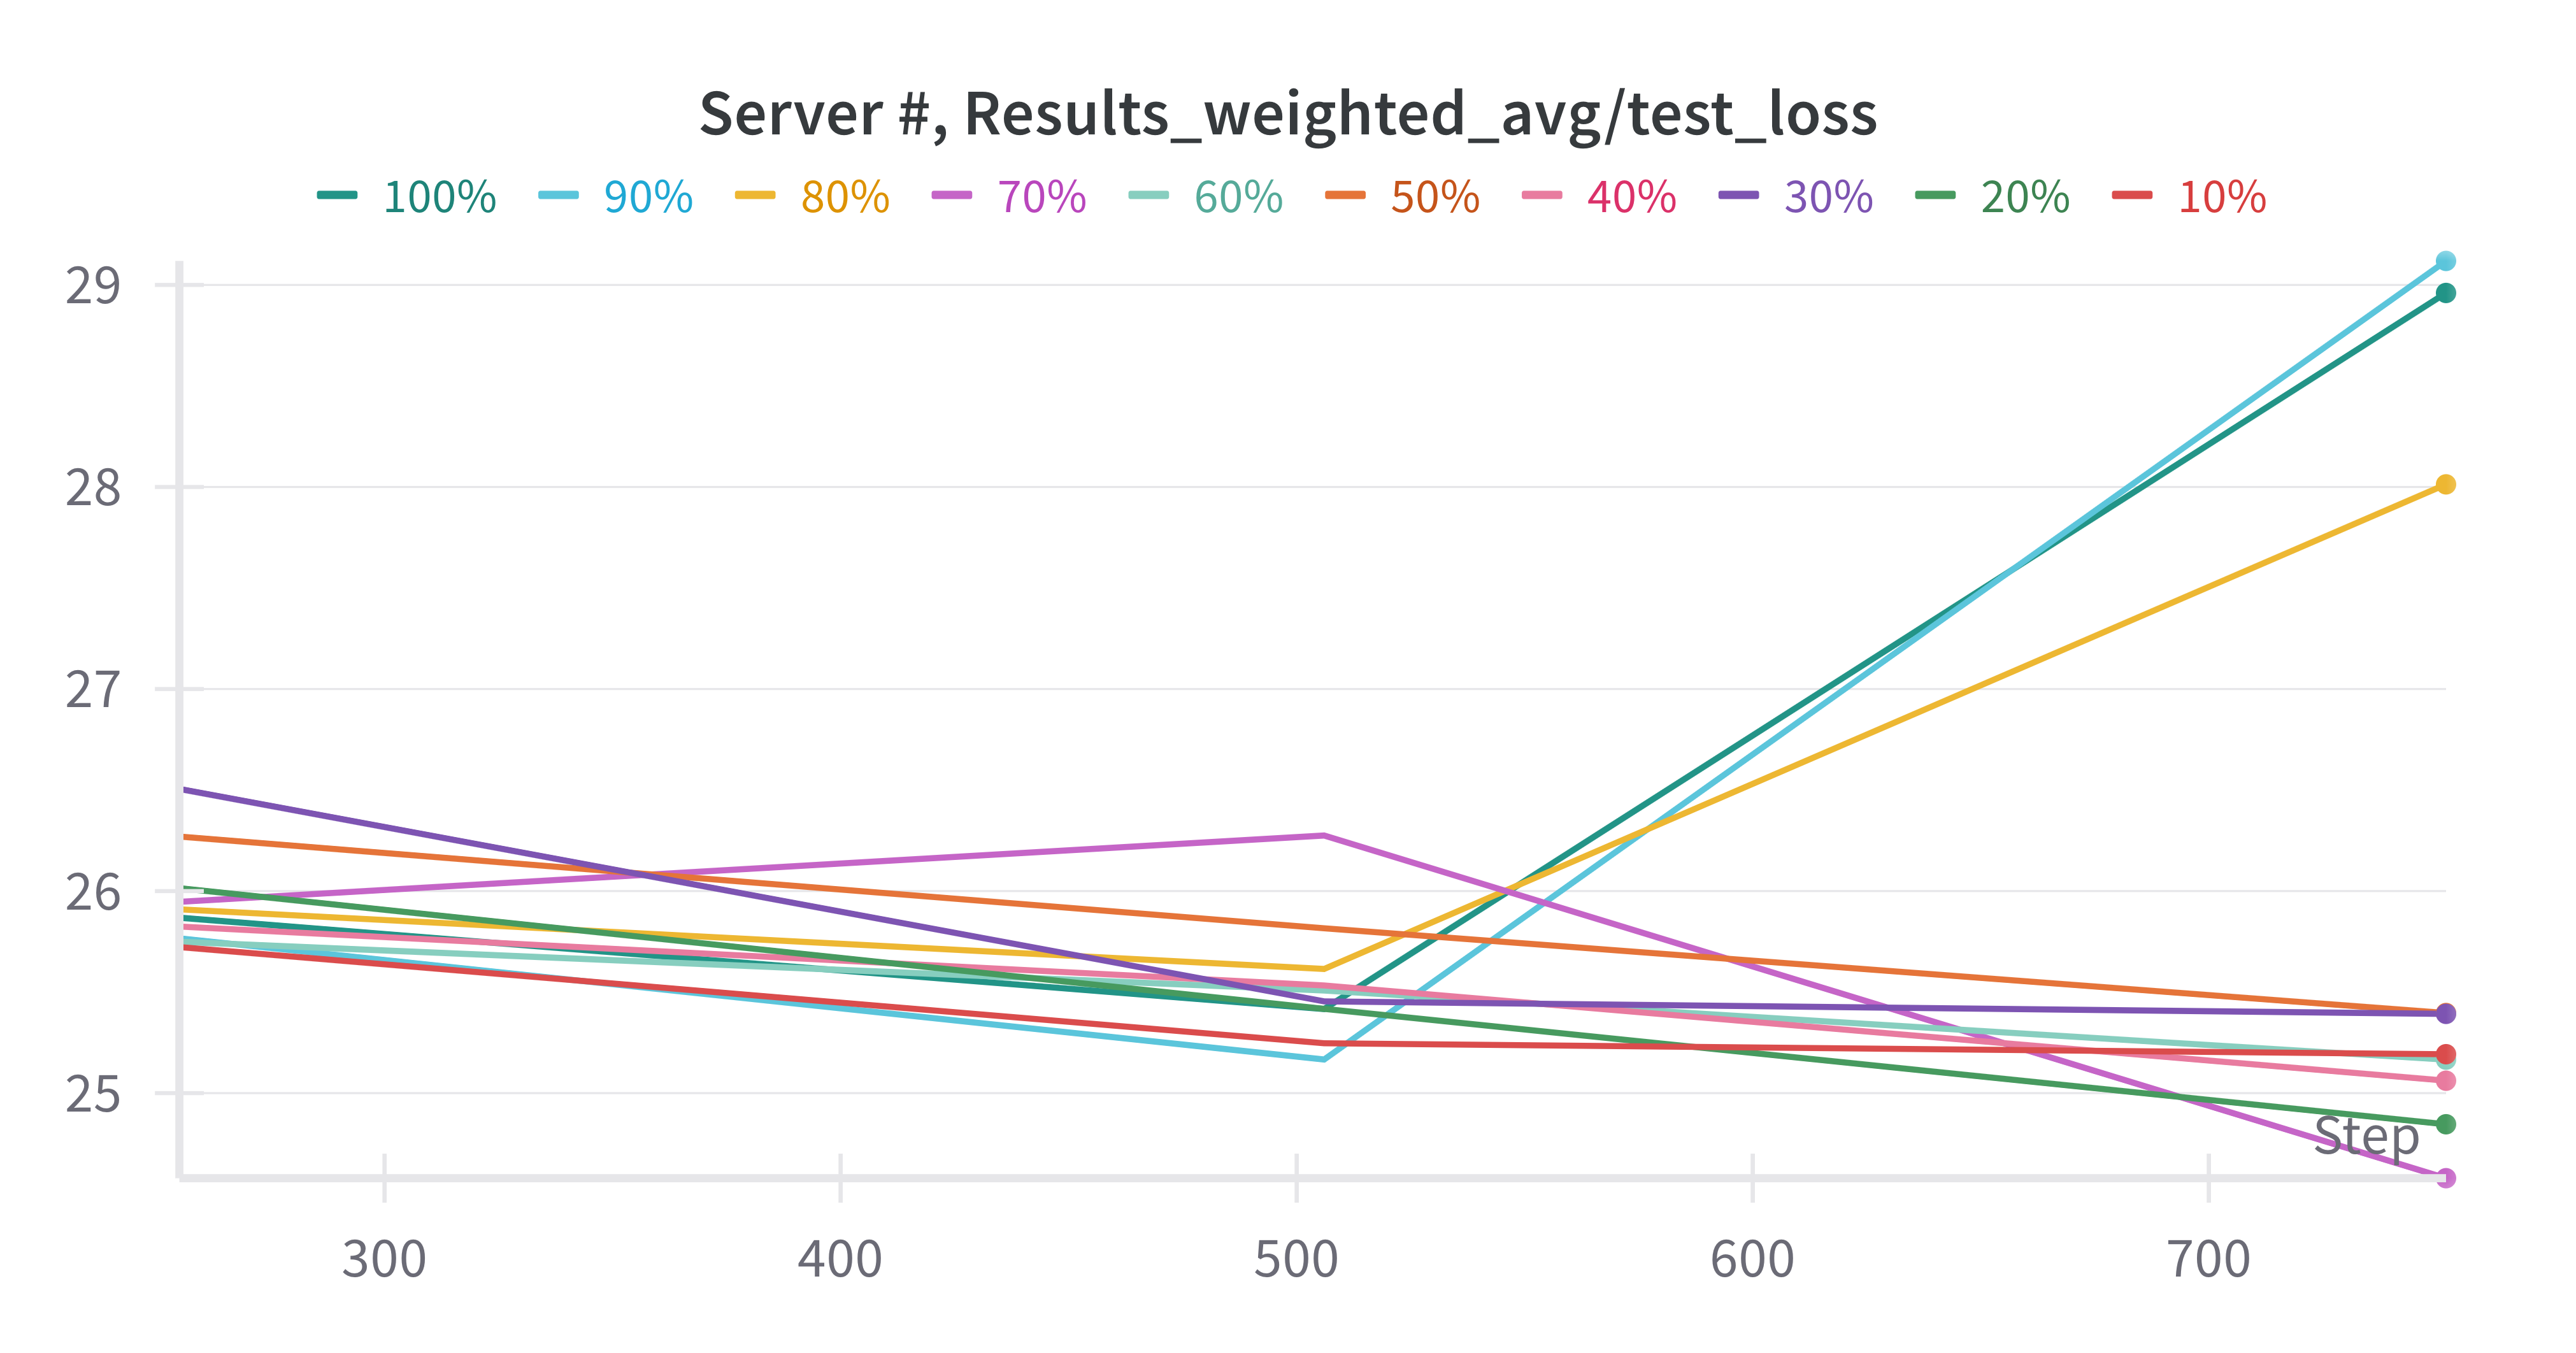
\includegraphics[width=\textwidth]{test_loss}
  \caption{Plot of the average test loss of the binary selectors across the different training set sizes.}
  \label{fig:t1}
\end{figure*}

For now, there isn’t much we can say, except that the training seems to be effective, as we see the accuracy increasing and the loss decreasing. Let’s wait for the RLHF results before drawing further conclusions.